\documentclass[journal,twoside,web]{ieeecolor}
\usepackage{jsen}
\usepackage{cite}
\usepackage{amsmath,amssymb,amsfonts}
\usepackage{algorithmic}
\usepackage{graphicx}
\usepackage{textcomp}
\usepackage{wrapfig}
\def\BibTeX{{\rm B\kern-.05em{\sc i\kern-.025em b}\kern-.08em
    T\kern-.1667em\lower.7ex\hbox{E}\kern-.125emX}}

\begin{document}
\title{CAB FARE PREDICTION USING HAVERSINE FORMULA}
\author{VinodkumarChintala (L00157096), Balasubramaniyam Muthuramalingam (L00157060), LYIT.
}

\maketitle

\section{Introduction}
\label{Introduction}
\IEEEPARstart

\\
\\

Artificial Intelligence (AI) is one of the emerging fields shaping the transportation sector. It is widely applied in public transportation, for example in cab services, companies use AI for calculating the distance from starting point to the end point and determine the price for the trip. Due to increase in demand of cabs, AI has shown significant development in this area. The distance is calculated by Haversine formula, given the latitude and longitude. The distance is directly proportional to the price, i.e., the value of the price increases with distance. By applying Decision Tree and Random forest tree and Linear Regression  algorithms, fare value for a trip is predicted. Further, to reduce the prediction error and to increase the accuracy speed Gradient Boosting technique is implemented. Setting up a target outcome for the future model will minimize the error. In order to setup a target outcome , for each iteration in the data depends on the amount of changes that affects the overall prediction error. If the change in prediction is small for a case it causes a large error drop so the predictions from the next model will produce values closer to target outcome which will reduce the error. Finally, if the small change of prediction causes no change in error, then the next outcome of the case is zero but it doesn’t mean it decreases the error.
At the end the model is optimized again using parameter tuning, hyperparameter optimization is implemented to customize the model to fit the dataset for a specific task. Hyperparameters are set manually by the user to guide the learning process. Two optimization algorithms are used to during hyperparameter tuning, Random Search and Grid Search. Random Search selects a domain which is also called a search space and randomly samples the points present in the domain. In Grid search the search spaces is defined by a grid and every position in the grid is evaluated. The performance is measured using an error whether it is minimized with zero error which represents it’s a perfect a model. Good performance are small negative values which is close to zero and perfect model is zero. Random search is preferred as it provides new hyperparameter values or new combination but grid search is quick to implement and appropriate for smaller datasets.
\\
\section{LITERATURE REVIEW:}
\label{LITERATURE REVIEW}
\\
There are reports related to the  models  predicting  the  price for cabs and other means of transportation systems. Anastasios Noulas’s group posted a paper in taxi price comparison exploiting their insights and challenges between Uber and Black cabs in mobile app. It showed that price charged by Uber were more stable than Black cabs as there were more deviations in Black cabs. It turns out Uber was stable when compared to Black cabs i.e., it provided accurate price for a trip without any surcharges most of the time. These prices are predicted with and without reduction co-efficient. There are four different factors involved in calculating the reduction co-efficient, availability, degree of necessity, time horizon and proportion of  budget.  Since  Black  cabs  prove to be more deviated so the price gain overall is calculated by taking the difference between Uber price and Black Cab price dividing by Black cab price.
\\
Another paper posted by Yash Indulkar, Analysis of Uber and Ola cabs using Deep Learning. Type of analysis is Sentiment Analysis; it is defined as the basic emotion of a human and trying to understand its problems. It focuses on understanding the customer’s complaint registered in Uber and Ola cab services and tweets, it is categorized as positive input or negative input. Two algorithms are used to determine the type of emotion/sentiment, Deep Feed forest neural network and Convolution neural network. Using the training dataset, the model is trained to and then tuned to work with testing dataset.
\\
A paper published by State Islamic University, shows the use of Haversine formula applied to count the visitor in an event. Haversine formula is used to calculate the distance between the user and the events that exist. The  existing  events are influenced by number of visitors registered in that geographic location . Using Location based service (LBS) user’s locations are saved, it’s a new technology used in Android applications. The result of Haversine is calculated with the radius of the area of event thus it can provide presence of visitors.
\\
\section{Datasets}
\label{Datasets}
\\
Datasets are contents of information stored in a tabular form. It is represented in .csv format. In this model two datasets are used; one is used for training  the  model  and other is used to test the model. The training dataset is used     to check if it is compatible with the respective algorithms, Decision tree, Random forest and Linear Regression algorithm. In the end it is optimized and processed using gradient boosting and parameter tuning.
\\
\subsection{Training Dataset}
\\
\\
In this dataset, the model is trained. The raw file is uploaded and analysed to understand the contents, total size of the data is 16074 entries and further categorized into rows and columns (16067 rows and 7 columns).
\\
There are 7  classes  of  different  datatypes.  6  Float  64  types and 1 Object types before pre-processing.
\\
\begin{center}
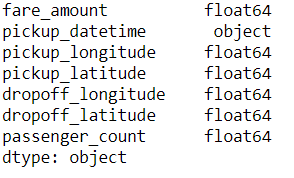
\includegraphics[scale=0.70]{Picture1.png}
\end{center}
\\
The below image is a sample set of information from the training dataset which is recorded from the year 2009 to 2015.
\\
\begin{center}
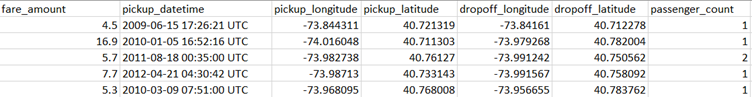
\includegraphics[scale=0.50]{Picture2.png}
\end{center}
\\
\subsection{Test Dataset:}
\\
\\
After training the model using the training dataset, the fare is predicted for the test dataset. This dataset for testing purpose and to check the accuracy of the model.  The fare is determined using the test dataset, it is tuned  further  for  accuracy.  There  are  9914  rows  and  6 columns. Each attribute is considered as classes with their own datatype (Object, Float64).
\\
\begin{center}
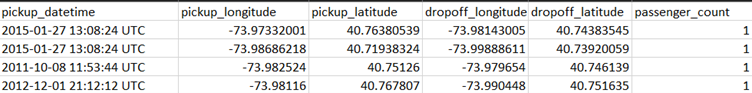
\includegraphics[scale=0.50]{Picture3.png}
\end{center}
\\
Sample entries of the dataset before processing.
\begin{center}
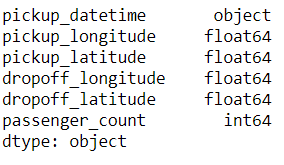
\includegraphics[scale=0.50]{Picture4.png}
\end{center}
\\
Attributes:-
\\
pickup date time: Starting time of cab ride.
\\
pickup longitude: Co-ordinate of pickup with respect to east and west
\\
pickup latitude: Co-ordinate of pickup with respect to north and south
\\
fare amount: Price for the trip 
\\
dropoff longitude: Co-ordinate of drop point with respect to east and west
\\
dropoff latitude: Co-ordinate of drop point with respect to north and south
\\
passenger count: number of passengers in a cab during the trip
\\
\\
\section{Methodology}
\label{Methodology}
\subsection{Overview:}
Cab price is determined by calculating the distance from starting point to ending point. It is a regression model, supervised learning. The datasets contain the latitude and longitude of the trips, using the co-ordinates we can determine the distance in kilometres(km). Using Haversine formula distance is calculated and stored in a new memory variable. Decision Tree algorithm, Linear Regression and Random forest algorithm is applied to train the model. This process is iterative until the model is familiar with the dataset, this helps the model to understand the task of the problem. Once the algorithm is applied to the model, mean squared error and R value are determined to predict the accuracy of the model and the deviation value or error value. Finally, the model is skimmed and optimized by tuning it. Gradient boosting and Parameter tuning are applied for the processed data to reduce the error rate and increase the speed of the accuracy i.e., the computation time required to provide the output. Under hyperparameter tuning two different optimization algorithms are applied, Grid Search and Random Search, this is done to measure the performance of the model using both the algorithm and after each iteration it records error value until it reaches zero which is considered as perfect model.
\\
\begin{center}
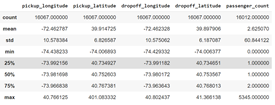
\includegraphics[scale=0.90]{Picture5.png}
\end{center}
\subsection{Latitude and Longitude:}
Latitude is geographic co-ordinates of north and south position on earth’s surface. The angle of latitude ranges between 0° and 90°. The circles parallel to the equator are constant lines of parallel, latitude is used together with longitude to find the accurate location. Longitude is like latitude, but it specifies the co-ordinates of east and west on earth’s surface. The angle of longitude  ranges  between  0° and 180°. The lines are represented in vertical with slight curvature.
\subsection{Pre-processing of Data:}
In this stage the datasets are observed and compared with the starting variable and target variable. If the data consists of any NaN values, it Is removed and aligned to provide a better presentation. While exploring the data, the following steps are involved, data cleaning [ dropping invalid values], data sorting, eliminating missing values and outlier analysis.
\subsection{Data Splitting:}
The training and testing dataset is split further for modelling,
\begin{center}
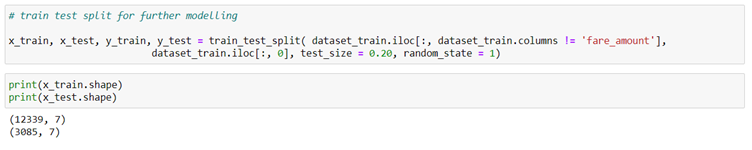
\includegraphics[scale=0.50]{Picture6.png}
\end{center}
\\
\subsection{Outlier Analysis:}
Values that exceeds the defined range are dropped along with the missing values. This phase is called the missing value analysis, where the dataset is observed to find  entries that does not enclose within the defined range. All the classes are analysed to check for NaN values and out of range values, the missing value percentage will increase if all the out of range values are defined as NaN which will lower the standard of dataset so to maintain the percentage of the missing values, out of range values are marked as outliers and removed using is.null() method.
\begin{center}
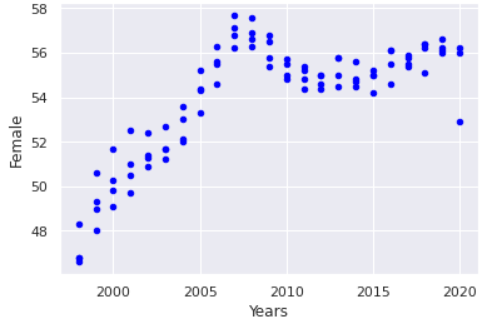
\includegraphics[scale=0.70]{Picture10.png}
\end{center}
\\
\subsection{Data Visualization:}
Data is represented in graph format,  this  is  used  to analytical and comparing purposes. Firstly, passenger count is represented, this is used to further to find the relation between the fare for a passenger with respect to the passenger count. 
\\
\begin{center}
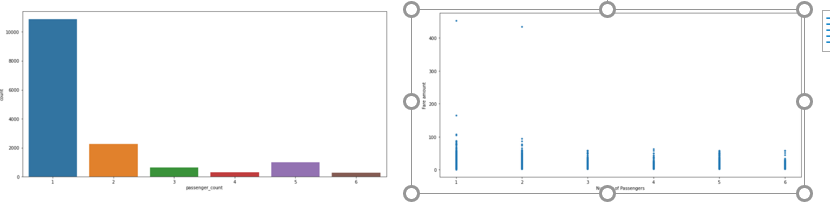
\includegraphics[scale=0.50]{Picture11.png}
\end{center}
The following observations are made:
\\
Passengers travelling alone or group of two are more frequent than others, i.e., passenger count for most of the entries is lesser than 3 but greater than 0.
Fare price are higher when passengers count is single or double.
The data is now further observed to check if the fare price is also dependent on date and time.
\begin{center}
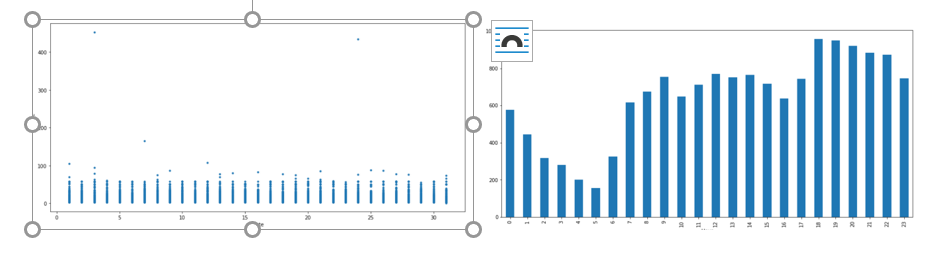
\includegraphics[scale=0.50]{Picture12.png}
\end{center}
\\
\section{ALGORITHMS USED}
\label{ALGORITHMS USED}
\subsection{Decision Tree Algorithm}
\\
Decision tree (DT) is a supervised learning, and it is used to solve classification and regression problems. It is a tree representation where each node is a class label. It has a root node and branch node. DT can represent any Boolean function on discrete values. After generating each set of branch nordes, DT struggles to choose  a root node for respective branches.
\\
There are two ways to determine the root node for branch nodes, Information Gain and Gini Index. Information gain, when a node is used in DT to split the training instances into smaller subsets, the randomness of the information changes i.e., entropy. It is defined as change in entropy, lower the change better to find the suitable root node.
\\
The data is split into two  axis,  x test  and  y test,  similarly for training dataset x train and y train. Calling Decision tree regressor to predict the data and stored in new variable.
\\
\begin{center}
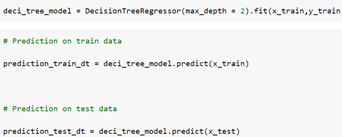
\includegraphics[scale=0.60]{Picture7.png}
\end{center}
\\
\subsection{Random Forest Algorithm}
\\
Random forest (RF) is made of trees and increased trees results in robust forest. Similarly, it creates decision trees on datasets and then gets the prediction from each node and finally selects the suited node by means of voting. It is an ensemble method which is better than a single decision tree because it reduces the over-fitting by averaging the result.
\\
\begin{center}
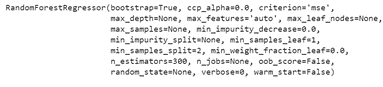
\includegraphics[scale=0.60]{Picture8.png}
\end{center}
\\
\begin{center}
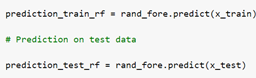
\includegraphics[scale=0.60]{Picture9.png}
\end{center}
\\
\\
\subsection{Linear Regression}
\\
Linear regression is a statistical model. It analyzes the linear relationship between two variables with a given set of dependent variables and independent variables. Linear relationship between variables is defined as the value of one or more independent variables will increase or decrease, the value of dependent variable will also increase or decrease accordingly. It can also be represented in mathematical terms : Y = mX+ b. The linear relationship between two variables can be positive or negative. Here, two attributes are assigned to X and Y coordinates, X as Years and Y as Male. A function is defined where the slope and intercept for the model is calculated.
\\
\begin{center}
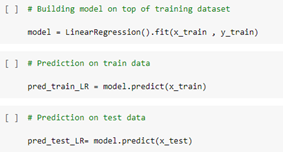
\includegraphics[scale=0.60]{Picture13new.png}
\end{center}
\\
\subsection{Gradient Boosting}
\\
It is a technique creating attention for the speed of accuracy and prediction and often used to optimize large and complex datasets. In gradient boosting the optimal solution is obtained by iterative process, the next best possible model and combined with the older model to reduce the prediction error. Target outcomes are set and calculated for each depending on how much the data prediction has changed and it impacts the overall prediction errors. If a small change causes large load on error, the target value is set to high. Otherwise, the model shows a small changes that causes no error, then the outcome for the next case is considered as zero. Changing the prediction does not decrement the error rate. Creating a Gradient model for training data and testing data and assigning to a new variable which is considered as a object to call the gradient model. Further we calculate the R value and Mean squared value to determine the error rate and accuracy of the model.
\\
\begin{center}
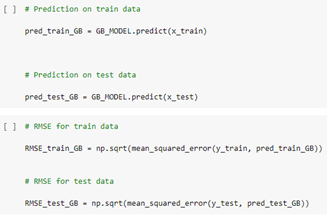
\includegraphics[scale=0.70]{Picture14new.png}
\end{center}
\\
\\
\subsection{Parameter Tuning}
Using hyperparameter tuning the model is customized for specific dataset. In hyperparameters the values are set manually to guide the learning process. In a model, it has wide range of hyperparameters and interact in a non-linear pattern. So it is required to search for perfect set of hyperparameters to provide an optimized solution for the model. It is done by applying optimizing algorithms Random Search and Grid Search.
\\
\begin{center}
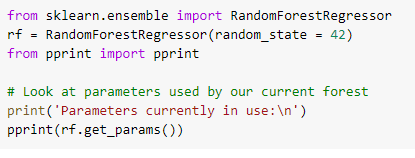
\includegraphics[scale=0.60]{Picture21.png}
\end{center}
\\
\\
\begin{center}
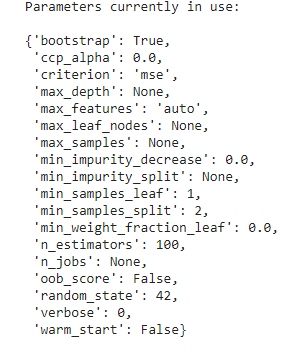
\includegraphics[scale=0.60]{Picture22.png}
\end{center}
\\
\subsection{Random Search}
It randomly samples points in the defined search space , It is applied by importing SickIt library , the model is evaluated for given set of hyperparameter vector using cross validation (CV). Two arguments are required to optimize the model, one is values of hyperparameter set and second is the search space which is called the domain. Applying random search CV in Random Forest
\\
\begin{center}
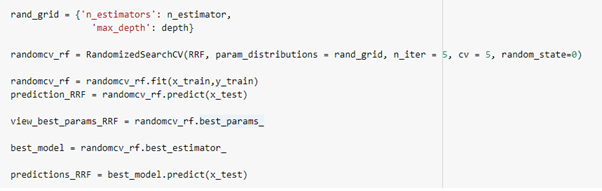
\includegraphics[scale=0.60]{Picture23.png}
\end{center}
\\
\subsection{Grid Search}
It evaluates every hyperparameter values in the grid within the search space. Grid search is efficient if the dataset isn’t complex and small. It is great for spot checking combination within the domain. Using grid search is like random forest. The only difference is the search space should be discrete grid to be searched. Importing grid search CV and assigning an object to it.
\\
\begin{center}
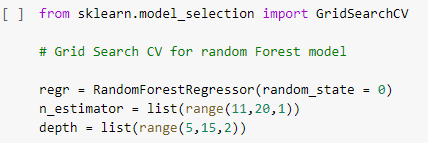
\includegraphics[scale=0.60]{Picture24.png}
\end{center}
\\
\\
\section{EVALUATION METRICS}
\label{EVALUATION METRICS}
\\
\\
Implementation of Haversine Formula:
\\
Haversine formula is an important equation to find the nav- igation, it gives shortest distance between two points on a sphere based on latitude and longitude. Importing math library under which sin, cos, sqrt, asin, radian methods are imported. After importing function is defined under which, co-ordinates of pickup latitude, pickup longititude and dropoff latitude, dropoff longitude, are stored in different memory indices. Converting units of latitude and longitude from degrees to radians.
\begin{center}
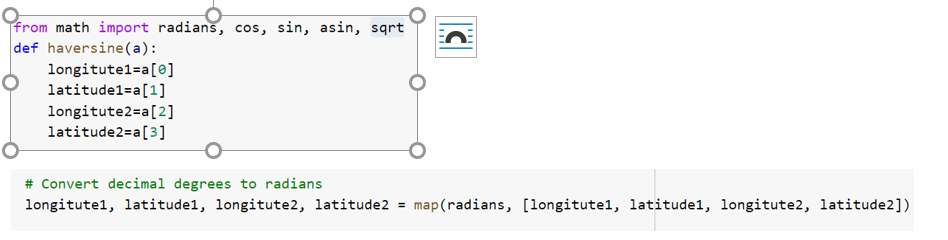
\includegraphics[scale=0.60]{Picture13.png}
\end{center}
Applying the haversine formula by finding the distance of longitude and latitudes. This is done by taking the difference between the end point and start point of longitude, similarly for latitude.
\\
The expression for haversine formula is d = 2r sin-1 sin²(2- 1/2) + cos 1 cos 2 sin²(2-1/2)
\begin{center}
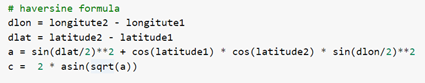
\includegraphics[scale=0.60]{Picture14.png}
\end{center}
\\
In the end, unit is converted to kilometre (km).
\\
\section{Result and Conclusion}
\label{Result and  Conclusion}
\\
Graph representation to define the relationship between the fare and distance which is calculated using haversine formuale.
\begin{center}
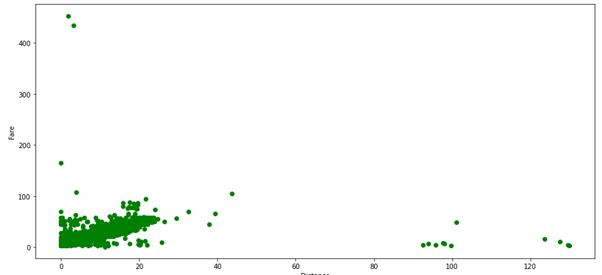
\includegraphics[scale=0.50]{Picture25.png}
\end{center}
\\
The dataset is compatible with the applied model, random forest, linear regression and decision tree, using the entries, R squared values were determined for both test and training dataset. The resulted value for both the datasets are below 1 for random forest, linear regression, decision tree. Mean squared error and Mean absolute error are calculated to evaluate the performance on the dataset before cleaned and processed.
\\
Mean Squared Error MSE
\\
Mean Absolute Error MAE
\\
R square for both test and train dataset
\\
R squared value is calculated after finding the mean squared error and mean absolute error for both the datasets.
\\
\\
Random Forest:  
\begin{center}
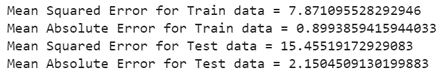
\includegraphics[scale=0.60]{Picture15.png}
\end{center}
\\
\\
R value for train data:
\begin{center}
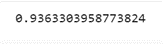
\includegraphics[scale=0.60]{Picture16.png}
\end{center}
\\
\\
R value for test data:
\begin{center}
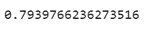
\includegraphics[scale=0.60]{Picture17.png}
\end{center}
\\
\\
Decision Tree:
\begin{center}
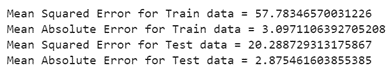
\includegraphics[scale=0.60]{Picture18.png}
\end{center}
\\
\\
\\
\\
R value for train data:
\begin{center}
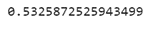
\includegraphics[scale=0.60]{Picture19.png}
\end{center}
\\
\\
R value for test data:
\begin{center}
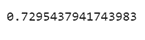
\includegraphics[scale=0.60]{Picture20.png}
\end{center}
\\
\\
Linear Regression:
\begin{center}
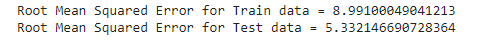
\includegraphics[scale=0.60]{Picture26.png}
\end{center}
\\
\\
R value for train Data:
\begin{center}
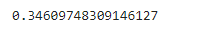
\includegraphics[scale=0.60]{Picture27.png}
\end{center}
\\
\\
R value for test Data:
\begin{center}
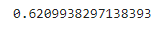
\includegraphics[scale=0.60]{Picture28.png}
\end{center}
\\
\\
Gradient Boosting Regressor:
\\
After using gradient boosting and finding the Mean Squared Value and R value for the train and test dataset.
\begin{center}
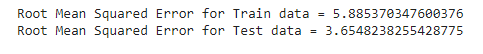
\includegraphics[scale=0.60]{Picture29.png}
\end{center}
\\
R value for train Data:
\begin{center}
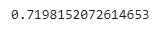
\includegraphics[scale=0.60]{Picture30.png}
\end{center}
\\
\\
R value for test Data:
\begin{center}
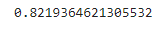
\includegraphics[scale=0.60]{Picture31.png}
\end{center}
\\
\\
Hyperparameter Tuning:
\\
\\
Random Forest using Cross Validation:
\\
After implementing hyperparameter tuning and determining the parameter to be used, Random Search hyperparameter Grid is created to calculate the R value and Mean squared Value.
\\
R value for train Data:
\begin{center}
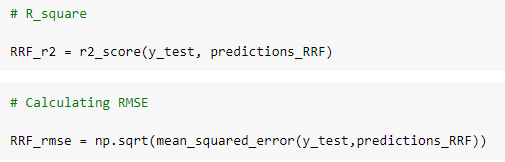
\includegraphics[scale=0.60]{Picture32.png}
\end{center}
\\
\\
R value for test Data:
\begin{center}
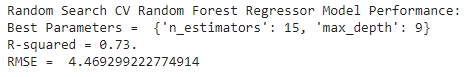
\includegraphics[scale=0.60]{Picture33.png}
\end{center}
\\
Applying the optimizing algorithm Random Search CV on Gradient boosting model and calculating the R value and Mean Squared value.
\\
\\
R value for test Data:
\begin{center}
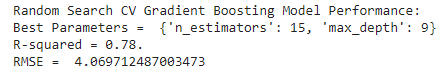
\includegraphics[scale=0.60]{Picture34.png}
\end{center}
\\
\\
\hspace{}
\\
Grid Search using Cross Validation with 5-Fold CV:
\\
R value for test Data:
\begin{center}
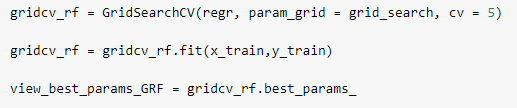
\includegraphics[scale=0.60]{Picture35.png}
\end{center}
\\
\\
R value for test Data:
\begin{center}
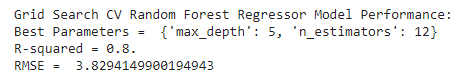
\includegraphics[scale=0.60]{Picture36.png}
\end{center}
\\
\\
Grid Search CV for Gradient Boosting:
\\
The R value and Mean Squared Value were determined using Random Forest CV on gradient boosting, now applying it using Grid Search CV with 5-Fold CV to determine the error.
\\
\begin{center}
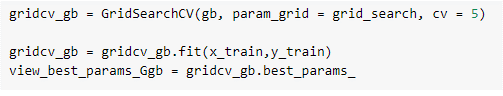
\includegraphics[scale=0.60]{Picture37.png}
\end{center}
\\
\\
\begin{center}
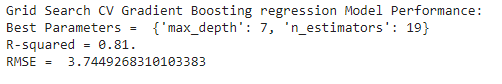
\includegraphics[scale=0.60]{Picture38.png}
\end{center}
\\
Fare Price using Grid Search CV.
\\
Comparing all the value shows that Grid Search is more opted as the value shows minimal error compared to Random Search CV on gradient boosting, hence choosing Grid Search optimizing on Random Forest Model using the test dataset to find the fare price for the calculated distance.
\\
\begin{center}
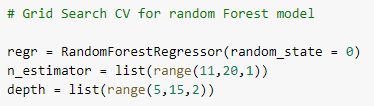
\includegraphics[scale=0.60]{Picture39.png}
\end{center}
\\
The data is already been cleaned and processed, hence applying grid search cv on the random forest model.
\\
\begin{center}
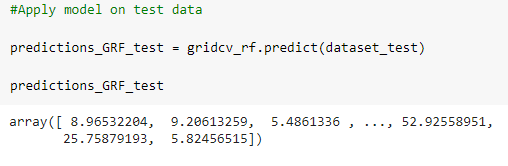
\includegraphics[scale=0.60]{Picture40.png}
\end{center}
\\
Final output for the test data after calculating the fare price using Grid Search
\\
\begin{center}
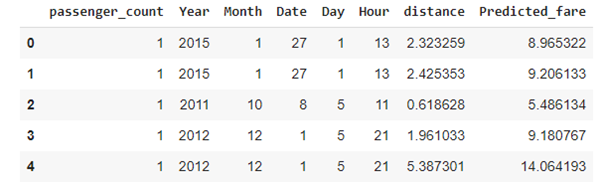
\includegraphics[scale=0.60]{Picture41.png}
\end{center}
\\
\\
\section{Future work}
\label{Future work}
\\
Finding optimal path for the given latitude and longitude can be done using Ant Colony optimization, it is specialized in solving the optimization problems , after each iteration the density of pheromone is vaporized. It represents the behavioural pattern of ants searching for food. This approach is carried out by a single ant wandering out for food and once it finds the source it traces back to its colony by leaving pheromone as a marker, using the marker the colony reaches the source. This marker is the path from the source to destination. It is an optimization technique for path finding algorithms, it provides increased accuracy i.e., it locates the exact position of the destination and calculates the total distance, which is the shortest path, hence it is more effective than haversine formulae.

\section{IMPORTANT LINKS}
\label{IMPORTANT LINKS}
\\
Data set link
https://www.kaggle.com/pankajkumar90/cab-fare-dataset
\\
Github link
https://github.com/TheAlgorithms


\begin{thebibliography}{00}
\\
\bibitem{b1}“Cecep Nurul Alam, Khaerul Manaf, Aldy Rialdy Atmadja, Digital Khrisna Aurum. Implementation of Haversine Formula for counting event visitor in radius based on Android Application. Informatics Engineering Dept Faculty of Science and Technology State Islamic University Sunan Gunung Jati Bandung].
\bibitem{b2}“2. Chopde, P.N.R., and Nichat, M.K. 2013. Landmark Based Shortest Path Detection by Using A* and Haversine Formula. Department of Computer Science and Engineering, G.H. Raisoni College of Engineer- ing and Management, Volume 1 Issue 2.].
\bibitem{b3}“3. Yash Indulkar,  Abhijit  Patil.  Sentiment  Analysis  of  Uber  and  Ola using Deep Learning. Information Technology Thakur College of Science Commerce.
\bibitem{b4}“4. Anastasios Noulas, Vsevolod Salnikov, Desislava Hristova, Cecilia Mascolo and Renaud Lambiotte. 2018. Developing and Deploying a Taxi Price Comparison Mobile App in the Wild: Insights and Challenges. Center for Data Science, New York University.
\bibitem{b5}[5]	A. Marazzi, “5. E. Alpaydin, Introduction to Machine Learning, 2nd ed. The MIT Press, 2010.
\bibitem{b6}[6]	“6. Kai Zhao1, Denis Khryashchev, Juliana Freire,Cl´audio Silva and Huy. Predicting Taxi Demand at High Spatial Resolution: Approaching the Limit of Predictability. Center for Urban Science and Progress, New York University 2Department of Computer Science and Engineering, New York University.
\bibitem{b7}https://towardsdatascience.com/introduction-to-machine-learningalgorithms-linear-regression-14c4e325882a
\bibitem{b8}Alper Sarikaya, Michael Correll, Lyn Bartram, Melanie Tory, and Danyel Fisher. (2018). What Do We Talk About When We Talk About Dashboards?. IEEE InfoVis 2018 (Berlin, Oct 21-26, 2018)
\bibitem{b9}https://www.decisionanalyst.com/media/downloads/ConsumerDecisionMaking.pdf
\bibitem{b10}Sengottuvelan P & Gopalakrishnan T (2016). A hybrid PSO with Naïve Bayes classifier for disengagement detection in online learning, Program, ISSN: 0033-0337, vol. 50, no. 2, pp. 215-224
\\
\bibitem{b11}https://machinelearningmastery.com/hyperparameter-optimization-with-random-search-and-grid-search/

\end{thebibliography}


\end{document}




